\section{Casi d'uso}

%contatore dei UserCases
\newcounter{CUC} % Contatore UserCases 
\newcounter{CSUC} % Contatore Sotto-UserCases
\newcounter{CSSUC} % Contatore Sotto-Sotto-UserCases
\newcommand{\stepUserCase}[0]{\stepcounter{CUC}\setcounter{CSUC}{0}\setcounter{CSSUC}{0}} % incrementa il contatore CUC
\newcommand{\stepsubUserCase}[0]{\stepcounter{CSUC}\setcounter{CSSUC}{0}} % incrementa il contatore CSUC
\newcommand{\stepsubsubUserCase}[0]{\stepcounter{CSSUC}} % incrementa il contatore CSSUC
\newcommand{\valueUserCase}[0]{UC\arabic{CUC} } % ritorna il valore del contatore CUC
\newcommand{\valuesubUserCase}[0]{UC\arabic{CUC}.\arabic{CSUC} } % ritorna il valore del contatore CSUC
\newcommand{\valuesubsubUserCase}[0]{UC\arabic{CUC}.\arabic{CSUC}.\arabic{CSSUC} } % ritorna il valore del contatore CSSUC
\newcommand{\resetCUC}[0]{\setcounter{CUC}{0}\setcounter{CSUC}{0}\setcounter{CSSUC}{0}}  % resetta il contatore CUC e CSUC
\newcommand{\labelUserCase}[0]{\label{UC\arabic{CUC}}}
\newcommand{\labelsubUserCase}[0]{\label{UC\arabic{CUC}.\arabic{CSUC}}}
\newcommand{\labelsubsubUserCase}[0]{\label{UC\arabic{CUC}.\arabic{CSUC}.\arabic{CSSUC}}}

\resetCUC

%1
\stepUserCase
\subsection{\valueUserCase - Visualizzazione home page}
\labelUserCase
\begin{itemize}
    \item \textbf{Attore primario:} cliente generico;
    \item \textbf{Descrizione:} il cliente apre il sito nella pagina principale;
    \item \textbf{Precondizione:} nessuna;
    \item \textbf{Input:} il cliente accede all'e-commerce tramite link diretto;
    \item \textbf{Postcondizione:} il cliente si trova nella pagina principale;
    \item \textbf{Scenario principale:} il cliente visualizza: elementi di identità del sito (logo, nome e-commerce), categorie presenti, prodotti in evidenza, informazioni sull'azienda venditrice (partita iva, indirizzo, ragione sociale, numero di telefono, email), pulsante per autenticarsi, pulsante per accedere al carrello.
\end{itemize}

%2
\stepUserCase
\subsection{\valueUserCase - Scelta categoria}
\labelUserCase
\begin{itemize}
    \item \textbf{Attore primario:} cliente generico;
    \item \textbf{Descrizione:} il cliente vuole visualizzare tutti i prodotti riguardanti una determinata categoria;
    \item \textbf{Precondizione:} il cliente si trova in una pagina dove la scelta di categoria è permessa;
    \item \textbf{Input:} seleziona una categoria;
    \item \textbf{Postcondizione:} il cliente visualizza tutti i prodotti relativi alla categoria selezionata;
    \item \textbf{Scenario principale:}
          \begin{enumerate}
              \item il cliente entra in una pagina dove è presente la scelta di una categoria;
              \item seleziona una categoria;
              \item viene reindirizzato ad una pagina di visualizzazione prodotto (PLP) e visualizza i prodotti desiderati (\hyperref[UC4]{UC4}).
          \end{enumerate}
\end{itemize}

%3
\stepUserCase
\subsection{\valueUserCase - Ricerca}
\labelUserCase
\begin{itemize}
    \item \textbf{Attore primario:} cliente generico;
    \item \textbf{Descrizione:} il cliente vuole visualizzare i prodotti che contengono nel nome prodotto una determinata parola;
    \item \textbf{Precondizione:} il cliente si trova in una pagina dove funzione di ricerca è permessa;
    \item \textbf{Input:} una stringa;
    \item \textbf{Postcondizione:} il cliente visualizza tutti i prodotti che contengono la determinata stringa nel nome;
    \item \textbf{Scenario principale:} il cliente entra in una pagina dove è permessa la ricerca di un prodotto, inserisce la parola da cercare e viene reindirizzato ad una pagina di visualizzazione prodotto (PLP) e visualizza i prodotti desiderati (\hyperref[UC4]{UC4}).
\end{itemize}

%4
\stepUserCase
\subsection{\valueUserCase - Visualizzazione lista prodotti (PLP)}
\labelUserCase
\begin{itemize}
    \item \textbf{Attore primario:} cliente generico;
    \item \textbf{Descrizione:} questa pagina visualizza tutti i prodotti che corrispondono ad una categoria o che corrispondono ad una parola cercata;
    \item \textbf{Precondizione:} il cliente sceglie uno dei due modi per accedere alla PLP (\hyperref[UC2]{UC2} e \hyperref[UC3]{UC3});
    \item \textbf{Postcondizione:} il cliente visualizza i prodotti che corrispondono alla scelta;
    \item \textbf{Scenario principale:}
          \begin{enumerate}
              \item il cliente può visualizzare tutti i prodotti che corrispondono alle politiche di visualizzazione;
              \item per ogni prodotto vengono visualizzati codice identificativo, titolo, foto principale e prezzo.
          \end{enumerate}
    \item \textbf{Estensioni:}
          \begin{itemize}
              \item la pagina visualizza una PLP vuota perché nessun prodotto corrisponde alle politiche di visualizzazione.
          \end{itemize}
\end{itemize}

%5
\stepUserCase
\subsection{\valueUserCase - Filtri}
\labelUserCase
\begin{itemize}
    \item \textbf{Attore primario:} cliente generico;
    \item \textbf{Descrizione:} il cliente può inserire ulteriori filtri per raffinare la visualizzazione dei prodotti;
    \item \textbf{Precondizione:} il cliente si deve trovare in una PLP (\hyperref[UC4]{UC4});
    \item \textbf{Postcondizione:} il cliente visualizza i prodotti con i filtri aggiornati;
    \item \textbf{Scenario principale:}
          \begin{enumerate}
              \item il cliente seleziona il filtro;
              \item il cliente modifica il valore del filtro;
              \item il cliente visualizza i prodotti secondo le nuove politiche;
          \end{enumerate}
    \item \textbf{Specializzazioni: }
          \begin{itemize}
              \item il cliente filtra i prodotti per prezzo (\hyperref[UC5.1]{UC5.1.});
              \item il cliente filtra i prodotti per categoria (\hyperref[UC5.2]{UC5.2}).
          \end{itemize}
\end{itemize}

%5.1
\stepsubUserCase
\subsubsection{\valuesubUserCase - Inserimento filtro prezzo}
\labelsubUserCase
\begin{itemize}
    \item \textbf{Attore primario:} cliente generico;
    \item \textbf{Descrizione:} questa funzionalità permette al cliente di filtrare i prodotti visualizzati per prezzo;
    \item \textbf{Precondizione:} il cliente si deve trovare in una PLP (\hyperref[UC4]{UC4});
    \item \textbf{Postcondizione:} il cliente visualizza i prodotti che corrispondono alla scelta;
    \item \textbf{Scenario principale:}
          \begin{enumerate}
              \item il cliente inserisce l'intervallo di prezzo desiderato;
              \item il cliente visualizza i prodotti che corrispondono alla scelta;
          \end{enumerate}
    \item \textbf{Estensioni:}
          \begin{itemize}
              \item la pagina visualizza una PLP vuota perché nessun prodotto corrisponde alle politiche di visualizzazione.
          \end{itemize}
\end{itemize}

%5.2
\stepsubUserCase
\subsubsection{\valuesubUserCase - Inserimento filtro categoria}
\labelsubUserCase
\begin{itemize}
    \item \textbf{Attore primario:} cliente generico;
    \item \textbf{Descrizione:} questa pagina visualizza tutti i prodotti che corrispondono ad una categoria o che corrispondono ad una parola cercata;
    \item \textbf{Precondizione:} il cliente sceglie uno dei due modi per accedere alla PLP (\hyperref[UC2]{UC2} e \hyperref[UC3]{UC3});
    \item \textbf{Postcondizione:} il cliente visualizza i prodotti che corrispondono alla scelta;
    \item \textbf{Scenario principale:}
          \begin{enumerate}
              \item il cliente seleziona una categoria;
              \item il cliente visualizza i prodotti che corrispondono alla scelta;
          \end{enumerate}
    \item \textbf{Estensioni:}
          \begin{itemize}
              \item la pagina visualizza una PLP vuota perché nessun prodotto corrisponde alle politiche di visualizzazione.
          \end{itemize}
\end{itemize}

%6
\stepUserCase
\subsection{\valueUserCase - Ordinamento prodotti per prezzo}
\labelUserCase
\begin{itemize}
    \item \textbf{Attore primario:} cliente generico;
    \item \textbf{Descrizione:} il cliente può ordinare i prodotti per prezzo crescente o decrescente;
    \item \textbf{Precondizione:} il cliente si deve trovare in una PLP (\hyperref[UC4]{UC4});
    \item \textbf{Postcondizione:} il cliente visualizza i prodotti ordinati;
    \item \textbf{Scenario principale:}
          \begin{enumerate}
              \item il cliente seleziona se ordinare per prezzo crescente (\hyperref[UC6.1]{UC6.1}) o decrescente (\hyperref[UC6.2]{UC6.2});
              \item il cliente visualizza la lista prodotti ordinata.
          \end{enumerate}
\end{itemize}

%6.1
\stepsubUserCase
\subsubsection{\valuesubUserCase - Ordinamento prezzo crescente}
\labelsubUserCase
\begin{itemize}
    \item \textbf{Attore primario:} cliente generico;
    \item \textbf{Descrizione:} il cliente vuole ordinare la lista per prezzo crescente;
    \item \textbf{Precondizione:} il cliente deve trovarsi nella PLP;
    \item \textbf{Postcondizione:} il cliente visualizza i prodotti in ordine crescente;
    \item \textbf{Scenario principale:}
          \begin{enumerate}
              \item il cliente seleziona l'ordinamento per prezzo crescente;
              \item il cliente visualizza i prodotti in ordine crescente;
          \end{enumerate}
\end{itemize}

%6.2
\stepsubUserCase
\subsubsection{\valuesubUserCase - Ordinamento prezzo decrescente}
\labelsubUserCase
\begin{itemize}
    \item \textbf{Attore primario:} cliente generico;
    \item \textbf{Descrizione:} il cliente vuole ordinare la lista per prezzo decrescente;
    \item \textbf{Precondizione:} il cliente deve trovarsi nella PLP;
    \item \textbf{Postcondizione:} il cliente visualizza i prodotti in ordine decrescente;
    \item \textbf{Scenario principale:}
          \begin{enumerate}
              \item il cliente seleziona l'ordinamento per prezzo decrescente;
              \item il cliente visualizza i prodotti in ordine decrescente;
          \end{enumerate}
\end{itemize}

%7
\stepUserCase
\subsection{\valueUserCase - Apertura pagina dettagli prodotto (PDP)}
\labelUserCase
\begin{itemize}
    \item \textbf{Attore primario:} cliente generico;
    \item \textbf{Descrizione:} questa pagina visualizza tutti i dettagli del prodotto;
    \item \textbf{Precondizione:} il cliente deve trovarsi in una pagina dove la visualizzazione dei dettagli del prodotto sia permessa;
    \item \textbf{Postcondizione:} il cliente visualizza tutti i dettagli del prodotto;
    \item \textbf{Scenario principale:}
          \begin{enumerate}
              \item il cliente visualizza il codice, il titolo, le foto, il prezzo e la descrizione del prodotto.
          \end{enumerate}
\end{itemize}

%8
\stepUserCase
\subsection{\valueUserCase - Aggiunta prodotto al carrello}
\labelUserCase
\begin{itemize}
    \item \textbf{Attore primario:} cliente generico;
    \item \textbf{Descrizione:} questa azione serve ad aggiungere un prodotto in vendita nel sito
          all'interno del carrello personale del cliente, specificando in quale quantità;
    \item \textbf{Precondizione:} il cliente si trova nella PDP di un prodotto (\hyperref[UC7]{UC7});
    \item \textbf{Input:} il cliente clicca sul pulsante "aggiungi al carrello" dopo aver selezionato la quantità (di default a 1);
    \item \textbf{Postcondizione:} l'oggetto è stato inserito nel carrello nella quantità desiderata (se disponibile in magazzino);
    \item \textbf{Scenario principale:}
          \begin{enumerate}
              \item il cliente seleziona la quantità desiderata o lascia quella di default (1);
              \item il cliente clicca sul pulsante "aggiungi al carrello".
          \end{enumerate}
    \item \textbf{Inclusioni:}
          \begin{itemize}
              \item viene eseguito un controllo sulla quantità disponibile di quel determinato prodotto;
          \end{itemize}
    \item \textbf{Estensioni:}
          \begin{itemize}
              \item in caso la quantità disponibile sia insufficiente a soddisfare la richiesta del cliente viene visualizzato un errore.
          \end{itemize}
\end{itemize}

%9
\stepUserCase
\subsection{\valueUserCase - Gestione carrello}
\labelUserCase
\begin{itemize}
    \item \textbf{Attore primario:} cliente generico;
    \item \textbf{Descrizione:} insieme di azioni fatte alla gestione degli articoli già presenti nel carrello;
    \item \textbf{Precondizione:} il cliente sta navigando il sito web;
    \item \textbf{Input:} il cliente esegue un'operazione gestionale sul carrello;
    \item \textbf{Postcondizione:} il cliente ha eseguito operazioni gestionali sul carrello;
    \item \textbf{Scenario principale:}
          \begin{enumerate}
              \item il cliente visualizza tutti gli articoli nel carrello (\hyperref[UC9.1]{UC9.1});
              \item il cliente può variare la quantità di ogni articolo (\hyperref[UC9.2]{UC9.2});
              \item il cliente può rimuovere un articolo dal carrello (\hyperref[UC9.3]{UC9.3}).
          \end{enumerate}
    
\end{itemize}

%9.1
\stepsubUserCase
\subsubsection{\valuesubUserCase - Visualizzazione articoli carrello}
\labelsubUserCase
\begin{itemize}
    \item \textbf{Attore primario:} cliente generico;
    \item \textbf{Descrizione:} scenario per la visualizzazione degli articoli nel carrello;
    \item \textbf{Precondizione:} il cliente si trova su una qualunque pagina del sito web;
    \item \textbf{Input:} il cliente preme su un pulsante dedicato all'accesso al carrello;
    \item \textbf{Postcondizione:} il cliente visualizza un resoconto di tutti i prodotti inseriti nel carrello durante la sessione di utilizzo corrente (se non autenticato), altrimenti il carrello mantiene la consistenza su ogni dispositivo fino al checkout.
    \item \textbf{Scenario principale:}
          \begin{enumerate}
              \item il cliente visualizza per ogni articolo codice, titolo, foto, prezzo e quantità;
              \item il cliente visualizza il totale dell'ordine con tasse incluse e senza costi di spedizione;
              \item il cliente visualizza il totale delle tasse.
          \end{enumerate}
    
\end{itemize}

%9.2
\stepsubUserCase
\subsubsection{\valuesubUserCase - Variazione quantità articolo}
\labelsubUserCase
\begin{itemize}
    \item \textbf{Attore primario:} cliente generico;
    \item \textbf{Descrizione:} scenario per la variazione della quantità di un singolo articolo presente nel carrello;
    \item \textbf{Precondizione:} il cliente ha eseguito (\hyperref[UC9.1]{UC9.1});
    \item \textbf{Input:} il cliente inserisce la nuova quantità desiderata per quel determinato articolo;
    \item \textbf{Postcondizione:} se la quantità desiderata è disponibile, viene aggiornato l'articolo nel carrello;
    \item \textbf{Scenario principale:}
          \begin{enumerate}
              \item il cliente seleziona la nuova quantità desiderata;
              \item il cliente conferma la scelta;
          \end{enumerate}
    \item \textbf{Inclusioni:}
          \begin{itemize}
              \item viene eseguito un controllo sulla quantità disponibile di quel determinato prodotto;
          \end{itemize}
    \item \textbf{Estensioni:}
          \begin{itemize}
              \item in caso la quantità disponibile sia insufficiente a soddisfare la richiesta del cliente viene visualizzato un errore.
          \end{itemize}
\end{itemize}

%9.3
\stepsubUserCase
\subsubsection{\valuesubUserCase - Rimozione articolo}
\labelsubUserCase
\begin{itemize}
    \item \textbf{Attore primario:} cliente generico;
    \item \textbf{Descrizione:} scenario per la rimozione di un articolo dal carrello;
    \item \textbf{Precondizione:} il cliente ha eseguito (\hyperref[UC9.1]{UC9.1});
    \item \textbf{Input:} il cliente preme su un pulsante dedicato alla rimozione di un determinato articolo dal carrello;
    \item \textbf{Postcondizione:} l'articolo selezionato non è più presente nel carrello.
\end{itemize}

%10
\stepUserCase
\subsection{\valueUserCase - Checkout}
\labelUserCase
\begin{figure}[H]
    \centering
    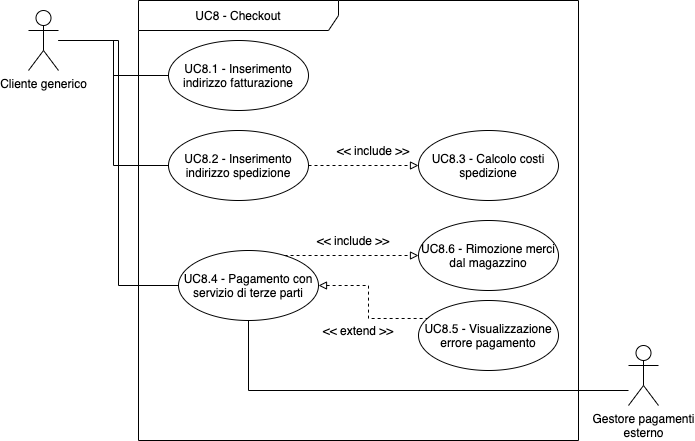
\includegraphics[width=\linewidth]{res/images/UC/UC8.png}
    \caption{Diagramma che descrive UC10 - Checkout}
\end{figure}
\begin{itemize}
    \item \textbf{Attore primario:} cliente generico;
    \item \textbf{Descrizione:} caso d'uso per l'acquisto dei prodotti inseriti nel carrello;
    \item \textbf{Precondizione:} il cliente ha eseguito (\hyperref[UC9.1]{UC9.1}) e il suo carrello contiene almeno un articolo;
    \item \textbf{Input:} il cliente preme sul pulsante per avviare il checkout;
    \item \textbf{Postcondizione:} viene emesso un ordine contenente gli articoli precedentemente inseriti nel carrello. Vengono quindi rimossi dal magazzino;
    \item \textbf{Scenario principale:}
          \begin{enumerate}
              \item il cliente preme sul pulsante per avviare il checkout;
              \item inserisce gli indirizzi di fatturazione e spedizione (\hyperref[UC10.1]{UC10.1} - \hyperref[UC10.2]{10.2});
              \item vengono aggiunti i costi della spedizione all'importo totale, definiti come importo fisso;
              \item si effettua il pagamento (\hyperref[UC10.3]{UC10.3});
              \item l'ordine è stato emesso e contrassegnato come pagato;
          \end{enumerate}
    \item \textbf{Estensioni:}
          \begin{itemize}
              \item in caso di fallimento del pagamento l'ordine non viene emesso, è necessario quindi riprovare il pagamento e viene visualizzato un errore;
              \item il cliente decide di annullare il processo di checkout premendo l'apposito pulsante.
          \end{itemize}
\end{itemize}

%10.1
\stepsubUserCase
\subsubsection{\valuesubUserCase - Inserimento indirizzo fatturazione}
\labelsubUserCase
\begin{itemize}
    \item \textbf{Attore primario:} cliente generico;
    \item \textbf{Descrizione:} scenario per l'inserimento dell'indirizzo di fatturazione in fase di checkout;
    \item \textbf{Precondizione:} il cliente ha avviato il processo di checkout;
    \item \textbf{Input:} il cliente inserisce i dati tramite l'apposito form oppure sceglie tra quelli personali già presenti (solo se autenticato);
    \item \textbf{Postcondizione:} il cliente procede con la fase successiva del checkout;
    \item \textbf{Scenario principale:}
          \begin{enumerate}
              \item il cliente ha 2 modi per inserire l'informazione:
                    \begin{itemize}
                        \item compilare il relativo form: nome, cognome, via/piazza, numero civico, codice avviamento postale, città, provincia, stato;
                        \item scegliere tra gli indirizzi salvati (solo se autenticato).
                    \end{itemize}
          \end{enumerate}
\end{itemize}

%10.2
\stepsubUserCase
\subsubsection{\valuesubUserCase - Inserimento indirizzo spedizione}
\labelsubUserCase
\begin{itemize}
    \item \textbf{Attore primario:} cliente generico;
    \item \textbf{Descrizione:} scenario per l'inserimento dell'indirizzo di spedizione in fase di checkout;
    \item \textbf{Precondizione:} il cliente ha avviato il checkout;
    \item \textbf{Input:} il cliente inserisce i dati tramite l'apposito form oppure sceglie tra quelli personali già presenti (solo se autenticato);
    \item \textbf{Postcondizione:} il cliente procede con la fase successiva del checkout;
    \item \textbf{Scenario principale:}
          \begin{enumerate}
              \item il cliente ha 3 modi per inserire l'informazione:
                    \begin{itemize}
                        \item compilare il relativo form: nome, cognome, via/piazza, numero civico, codice avviamento postale, città, provincia, stato;
                        \item scegliere tra gli indirizzi salvati (solo se autenticato);
                        \item riutilizzare l'indirizzo di fatturazione precedentemente inserito.
                    \end{itemize}
          \end{enumerate}
\end{itemize}

%10.3
\stepsubUserCase
\subsubsection{\valuesubUserCase - Pagamento con servizio di terze parti}
\labelsubUserCase
\begin{itemize}
    \item \textbf{Attore primario:} cliente generico;
    \item \textbf{Attore secondario:} gestore dei pagamenti esterno;
    \item \textbf{Descrizione:} scenario per il pagamento del totale dell'ordine mediante un gestore di pagamenti esterno a EmporioLambda;
    \item \textbf{Precondizione:} sono stati eseguiti tutti i passi precedenti del checkout, ovvero sono stati applicati i costi della spedizione al totale;
    \item \textbf{Input:} il cliente preme sul pulsante per pagare;
    \item \textbf{Postcondizione:} il pagamento è stato eseguito e l'ordine viene emesso. Vengono quindi rimosse dal magazzino le merci acquistate;
    \item \textbf{Scenario principale:}
          \begin{enumerate}
              \item il cliente premendo sul pulsante per eseguire il pagamento viene rimandato alla piattaforma esterna;
              \item esegue il pagamento interagendo con il servizio esterno;
              \item in caso di pagamento riuscito l'ordine viene emesso e le merci acquistate vengono rimosse dal magazzino;
          \end{enumerate}
    \item \textbf{Estensioni:}
          \begin{itemize}
              \item in caso di pagamento fallito viene visualizzato un errore e si offre la possibilità di riprovare premendo di nuovo sul tasto per eseguire il pagamento.
          \end{itemize}
\end{itemize}

%11
\stepUserCase
\subsection{\valueUserCase - Login cliente}
\labelUserCase
\begin{itemize}
    \item \textbf{Attore primario:} cliente non autenticato;
    \item \textbf{Attore secondario:} gestore delle credenziali esterno;
    \item \textbf{Descrizione:} caso d'uso per l'autenticazione del cliente;
    \item \textbf{Precondizione:} il cliente non si è ancora autenticato nell'applicazione;
    \item \textbf{Input:} il cliente inserisce ed invia i dati per il login;
    \item \textbf{Postcondizione:} il cliente è autenticato;
    \item \textbf{Scenario principale:}
          \begin{enumerate}
              \item il cliente inserisce username e password;
              \item invia i dati inseriti;
              \item i dati vengono verificati dal gestire esterno;
              \item se i dati sono corretti e identificato un profilo utente il cliente è autenticato con questo profilo;
          \end{enumerate}
    \item \textbf{Estensioni:}
          \begin{enumerate}
              \item il gestore delle credenziali restituisce un errore indicante che i dati inseriti sono errati;
              \item viene quindi chiesto di reinserire le credenziali, contestualmente si visualizza un messaggio di errore.
          \end{enumerate}
\end{itemize}

%12
\stepUserCase
\subsection{\valueUserCase - Registrazione cliente}
\labelUserCase
\begin{itemize}
    \item \textbf{Attore primario:} cliente non autenticato;
    \item \textbf{Attore secondario:} gestore delle credenziali esterno;
    \item \textbf{Descrizione:} caso d'uso per la registrazione di un nuovo cliente;
    \item \textbf{Precondizione:} il cliente non si è ancora autenticato nell'applicazione;
    \item \textbf{Input:} il cliente inserisce ed invia i dati per la registrazione;
    \item \textbf{Postcondizione:} il cliente è autenticato con il nuovo profilo appena inserito nel sistema;
    \item \textbf{Scenario principale:}
          \begin{enumerate}
              \item il cliente inserisce l'email, la quale verrà utilizzata per contattarlo e per identificare univocamente l'utente nel sistema;
              \item il cliente reinserisce l'email per conferma;
              \item il cliente inserisce una password che rispetti i requisiti minimi di sicurezza;
              \item il cliente reinserisce la stessa password per conferma.
              \item i dati vengono inviati al servizio di terze parti per la gestione dei dati di login;
              \item arriva un'email al cliente contenente un link per la verifica all'indirizzo indicato;
              \item il cliente deve premere su quel link per attivare l'account entro una finestra di tempo limitata.
          \end{enumerate}
    \item \textbf{Estensioni:} la registrazione fallisce se:
          \begin{itemize}
              \item nel sistema esiste già un cliente con la stessa email;
              \item le due email inserite non corrispondono;
              \item le due password inserite non corrispondono;
              \item il cliente non preme il link di verifica inviato alla sua casella di posta.
          \end{itemize}
\end{itemize}

%13
\stepUserCase
\subsection{\valueUserCase - Reimpostazione password cliente}
\labelUserCase
\begin{itemize}
    \item \textbf{Attore primario:} cliente non autenticato;
    \item \textbf{Attore secondario:} gestore delle credenziali esterno;
    \item \textbf{Descrizione:} caso d'uso per la reimpostazione della password, utile quando il cliente la dimentica;
    \item \textbf{Precondizione:} il cliente non si è ancora autenticato nell'applicazione e si trova nella pagina di login;
    \item \textbf{Input:} il cliente preme sul pulsante per la reimpostazione della password;
    \item \textbf{Postcondizione:} il cliente ha modificato la sua password e può effettuare il login;
    \item \textbf{Scenario principale:}
          \begin{enumerate}
              \item il cliente chiede la reimpostazione della password;
              \item riceve tramite email un link per la reimpostazione valido entro un certo limite di tempo;
              \item preme sul link e viene portato su una pagina per l'inserimento della password;
              \item inserisce la nuova password;
              \item reinserisce la password per conferma;
              \item invia i dati inseriti al gestore delle credenziali.
          \end{enumerate}
    \item \textbf{Estensioni:} la reimpostazione della password fallisce se:
          \begin{itemize}
              \item le password inserite non corrispondono;
              \item la nuova password non rispetta i requisiti minimi di sicurezza.
          \end{itemize}
\end{itemize}

%14
\stepUserCase
\subsection{\valueUserCase - Amministrazione account}
\labelUserCase
\begin{figure}[H]
    \centering
    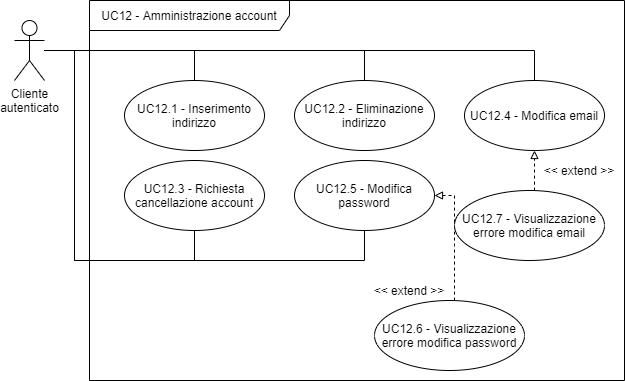
\includegraphics[width=\linewidth]{res/images/UC/UC12.png}
    \caption{Diagramma che descrive UC14 - Amministrazione account}
\end{figure}
\begin{itemize}
    \item \textbf{Attore primario:} cliente autenticato;
    \item \textbf{Descrizione:} caso d'uso per la gestione del profilo utente di un cliente;
    \item \textbf{Precondizione:} il cliente ha eseguito il login (\hyperref[UC11]{UC11}) e si trova sulla pagina per la gestione del profilo;
    \item \textbf{Input:} il cliente avvia un'operazione di gestione profilo;
    \item \textbf{Postcondizione:} il cliente ha modificato il suo profilo o richiesto la modifica al venditore.
    \item \textbf{Scenario principale:}
          \begin{enumerate}
              \item il cliente può inserire un nuovo indirizzo (\hyperref[UC14.1]{UC14.1});
              \item il cliente può eliminare un indirizzo presente (\hyperref[UC14.2]{UC14.2});
              \item il cliente può richiedere la cancellazione dell'account (\hyperref[UC14.3]{UC14.3});
              \item il cliente può modificare la propria email (\hyperref[UC14.4]{UC14.4});
              \item il cliente può modificare la propria password (\hyperref[UC14.5]{UC14.5}).
            
          \end{enumerate}
\end{itemize}

%14.1
\stepsubUserCase
\subsubsection{\valuesubUserCase - Inserimento indirizzo}
\labelsubUserCase
\begin{itemize}
    \item \textbf{Attore primario:} cliente autenticato;
    \item \textbf{Descrizione:} scenario per l'inserimento di un nuovo indirizzo (utilizzabile per spedizione e/o fatturazione in fase di checkout);
    \item \textbf{Precondizione:} il cliente ha eseguito il login (\hyperref[UC11]{UC11}) e si trova sulla pagina per la gestione del profilo;
    \item \textbf{Input:} il cliente seleziona l'opzione per inserire un nuovo indirizzo;
    \item \textbf{Postcondizione:} nel sistema esiste l'indirizzo inserito dal cliente;
    \item \textbf{Scenario principale:}
          \begin{enumerate}
              \item il cliente compila il form per l'inserimento dell'indirizzo: nome, cognome, via/piazza, numero civico, codice avviamento postale, città, provincia, stato;
              \item il cliente invia quindi i dati.
          \end{enumerate}
\end{itemize}

%14.2
\stepsubUserCase
\subsubsection{\valuesubUserCase - Eliminazione indirizzo}
\labelsubUserCase
\begin{itemize}
    \item \textbf{Attore primario:} cliente autenticato;
    \item \textbf{Descrizione:} scenario per l'eliminazione di un indirizzo precedentemente inserito;
    \item \textbf{Precondizione:} il cliente ha eseguito il login (\hyperref[UC11]{UC11}) e si trova sulla pagina per la gestione del profilo;
    \item \textbf{Input:} il cliente seleziona l'opzione per eliminare un indirizzo;
    \item \textbf{Postcondizione:} nel sistema non esiste più l'indirizzo rimosso.
\end{itemize}

%14.3
\stepsubUserCase
\subsubsection{\valuesubUserCase - Richiesta cancellazione account}
\labelsubUserCase
\begin{itemize}
    \item \textbf{Attore primario:} cliente autenticato;
    \item \textbf{Descrizione:} scenario per la richiesta di cancellazione del profilo cliente al venditore;
    \item \textbf{Precondizione:} il cliente ha eseguito il login (\hyperref[UC11]{UC11}) e si trova sulla pagina per la gestione del profilo;
    \item \textbf{Input:} il cliente preme il pulsante per richiedere la cancellazione dell'account;
    \item \textbf{Postcondizione:} il sistema invia una email predefinita al venditore contenente la richiesta di cancellazione del relativo account.
\end{itemize}

%14.4
\stepsubUserCase
\subsubsection{\valuesubUserCase - Modifica email}
\labelsubUserCase
\begin{itemize}
    \item \textbf{Attore primario:} cliente autenticato;
    \item \textbf{Descrizione:} scenario per la modifica dell'email (username) dell'utente;
    \item \textbf{Precondizione:} il cliente ha eseguito il login (\hyperref[UC11]{UC11}) e si trova sulla pagina per la gestione del profilo;
    \item \textbf{Input:} il cliente sceglie l'opzione per modificare l'email che lo identifica univocamente all'interno del sito;
    \item \textbf{Postcondizione:} l'email è stata modificata con quella nuova inserita;
    \item \textbf{Scenario principale:}
          \begin{enumerate}
              \item il cliente inserisce l'email nel campo apposito;
              \item il cliente reinserisce la stessa email in un altro campo per la verifica;
              \item il cliente invia quindi i dati inseriti;
              \item si ripete il processo di verifica email spiegato nel caso d'uso della registrazione.
          \end{enumerate}
    \item \textbf{Estensioni:} la modifica dell'email fallisce se:
          \begin{itemize}
              \item i due indirizzi email non corrispondono;
              \item il nuovo indirizzo non viene verificato.
          \end{itemize}
\end{itemize}

%14.5
\stepsubUserCase
\subsubsection{\valuesubUserCase - Modifica password}
\labelsubUserCase
\begin{itemize}
    \item \textbf{Attore primario:} cliente autenticato;
    \item \textbf{Descrizione:} scenario per la modifica della password del cliente;
    \item \textbf{Precondizione:} il cliente ha eseguito il login (\hyperref[UC11]{UC11}) e si trova sulla pagina per la gestione del profilo;
    \item \textbf{Input:} il cliente seleziona l'opzione per modificare la password di accesso;
    \item \textbf{Postcondizione:} la password di accesso al sistema per quel cliente è stata modificata;
    \item \textbf{Scenario principale:}
          \begin{enumerate}
              \item il cliente inserisce la vecchia password;
              \item il cliente inserisce la nuova password;
              \item il cliente reinserisce la nuova password;
              \item il cliente invia quindi i dati inseriti.
          \end{enumerate}
    \item \textbf{Estensioni:} la modifica della password fallisce se:
          \begin{itemize}
              \item le password inserite non corrispondono;
              \item la nuova password non rispetta i requisiti minimi di sicurezza.
          \end{itemize}
\end{itemize}

%15
\stepUserCase
\subsection{\valueUserCase - Gestione ordini cliente}
\labelUserCase
\begin{itemize}
    \item \textbf{Attore primario:} cliente autenticato;
    \item \textbf{Descrizione:} il cliente vuole accedere all'area di gestione degli ordini;
    \item \textbf{Precondizione:} il cliente è autenticato nel sito;
    \item \textbf{Postcondizione:} il cliente risulta nella pagina dove è possibile gestire gli ordini effettuati;
    \item \textbf{Input:} il cliente preme il pulsante per visualizzare la lista degli ordini;
    \item \textbf{Scenario principale:}
          \begin{enumerate}
              \item il cliente può annullare l'ordine (\hyperref[UC15.1]{UC15.1});
              \item il cliente può richiedere assistenza per un ordine (\hyperref[UC15.2]{UC15.2});
              \item il cliente può richiedere un reso (\hyperref[UC15.3]{UC15.3});
              \item il cliente può visualizzare il riepilogo di un determinato ordine (\hyperref[UC15.4]{UC15.4});
              \item il cliente può visualizzare la pagina con la lista degli ordini (\hyperref[UC15.4]{UC15.4}).
          \end{enumerate}
\end{itemize}

%15.1
\stepsubUserCase
\subsubsection{\valuesubUserCase - Annullamento ordine}
\labelsubUserCase
\begin{itemize}
    \item \textbf{Attore primario:} cliente autenticato;
    \item \textbf{Descrizione:} il cliente vuole annullare un ordine effettuato;
    \item \textbf{Precondizione:} il cliente deve aver effettuato un ordine e trovarsi nella sezione gestione degli ordini e visualizzare il dettaglio di un ordine (\hyperref[UC15.4]{UC15.4});
    \item \textbf{Input:} il cliente clicca sul pulsante per l'annullamento dell'ordine;
    \item \textbf{Postcondizione:} il cliente ha contatto il venditore per l'annullamento;
    \item \textbf{Scenario principale:}
          \begin{enumerate}
              \item il cliente sceglie ordine da annullare;
              \item il cliente viene portato al form di contatto dove sarà già precompilato il numero dell'ordine che si desidera annullare;
              \item il cliente seleziona il motivo dell'annullamento;
              \item il cliente scrive un messaggio per il venditore.
          \end{enumerate}
    \item \textbf{Inclusioni:}
          \begin{itemize}
              \item per annullare un ordine viene aperto il form di contatto che permette al cliente di contattare il venditore (\hyperref[UC17]{UC17}).
          \end{itemize}
\end{itemize}

%15.2
\stepsubUserCase
\subsubsection{\valuesubUserCase - Assistenza cliente}
\labelsubUserCase
\begin{itemize}
    \item \textbf{Attore primario:} cliente autenticato;
    \item \textbf{Descrizione:} il cliente vuole contattare il venditore per un problema (errore indirizzo, domande, etc.);
    \item \textbf{Precondizione:} il cliente deve trovarsi nella pagina della gestione degli ordini, aver effettuato l'ordine e visualizzarne il riepilogo (\hyperref[UC15.4]{UC15.4});
    \item \textbf{Input:} il cliente clicca sul pulsante per l'assistenza;
    \item \textbf{Postcondizione:} il cliente ha contatto il venditore per richiedere assistenza;
    \item \textbf{Scenario principale:}
          \begin{enumerate}
              \item il cliente decide di contattare l'assistenza;
              \item il cliente viene portato al form di contatto dove sarà già precompilato il numero dell'ordine al quale si desidera chiedere assistenza;
          \end{enumerate}
    \item \textbf{Inclusioni:}
          \begin{itemize}
              \item per l'assistenza su un ordine viene aperto il form di contatto che permette al cliente di contattare il venditore (\hyperref[UC17]{UC17}).
          \end{itemize}
\end{itemize}

%15.3
\stepsubUserCase
\subsubsection{\valuesubUserCase - Richiesta reso}
\labelsubUserCase
\begin{itemize}
    \item \textbf{Attore primario:} cliente autenticato;
    \item \textbf{Descrizione:} il cliente vuole effettuare un reso di un ordine ricevuto;
    \item \textbf{Precondizione:} il cliente deve aver effettuato un ordine, averlo ricevuto, ed essere nella pagina di visualizzazione dettaglio (\hyperref[UC15.4]{UC15.4});
    \item \textbf{Input:} il cliente clicca sul pulsante per il reso dell'ordine;
    \item \textbf{Postcondizione:} il cliente ha contatto il venditore per il reso;
    \item \textbf{Scenario principale:}
          \begin{enumerate}
              \item il cliente decide di effettuare un reso;
              \item il cliente viene portato al form di contatto dove sarà già precompilato il numero dell'ordine di cui si desidera effettuare il reso;
          \end{enumerate}
    \item \textbf{Inclusioni:}
          \begin{itemize}
              \item per il reso di un ordine viene aperto il form di contatto che permette al cliente di contattare il venditore (\hyperref[UC17]{UC17}).
          \end{itemize}
\end{itemize}

%15.4
\stepsubUserCase
\subsubsection{\valuesubUserCase - Riepilogo ordine}
\labelsubUserCase
\begin{itemize}
    \item \textbf{Attore primario:} cliente autenticato;
    \item \textbf{Descrizione:} il cliente vuole visualizzare il riepilogo dell'ordine effettuato;
    \item \textbf{Precondizione:} il cliente ha effettuato l'ordine e deve trovarsi nella pagina di gestione degli ordini;
    \item \textbf{Input:} il cliente clicca sul pulsante per la visualizzazione del riepilogo dell'ordine;
    \item \textbf{Postcondizione:} il cliente visualizza il riepilogo;
    \item \textbf{Scenario principale:}
          \begin{enumerate}
              \item il cliente decide di aprire il riepilogo dell'ordine;
              \item si apre la pagina dove è presentato il riepilogo: numero identificativo, data, importo totale, prodotti acquistati (per ognuno codice, titolo, prezzo e quantità), indirizzo di fatturazione e spedizione, stato dell'ordine.
          \end{enumerate}
\end{itemize}

%15.5
\stepsubUserCase
\subsubsection{\valuesubUserCase - Visualizzazione lista ordini}
\labelsubUserCase
\begin{itemize}
    \item \textbf{Attore primario:} cliente autenticato;
    \item \textbf{Descrizione:} il cliente vuole visualizzare tutti gli ordini da lui effettuati;
    \item \textbf{Precondizione:} il cliente si trova nella sezione di gestione ordini;
    \item \textbf{Input:} il cliente clicca sul pulsante per visualizzare gli ordini;
    \item \textbf{Postcondizione:} il cliente visualizza tutti gli ordini effettuati in maniera sintetica;
    \item \textbf{Scenario principale:}
          \begin{enumerate}
              \item il cliente decide di aprire la lista ordini;
              \item si apre la pagina contenente la lista degli ordini effettuati: per ognuno si visualizza data, totale, numero totale di articoli acquistati, numero identificativo dell'ordine, stato dell'ordine.
          \end{enumerate}
\end{itemize}

%16
\stepUserCase
\subsection{\valueUserCase - Logout cliente}
\labelUserCase
\begin{itemize}
    \item \textbf{Attore primario:} cliente autenticato;
    \item \textbf{Descrizione:} il cliente vuole effettuare il logout;
    \item \textbf{Precondizione:} il cliente è autenticato al sito;
    \item \textbf{Input:} il cliente clicca sul pulsante per il logout;
    \item \textbf{Postcondizione:} il cliente risulta non autenticato nel sito;
    \item \textbf{Scenario principale:}
          \begin{enumerate}
              \item il cliente effettua il logout;
              \item il cliente si ritrova nella pagina principale del sito.
          \end{enumerate}
\end{itemize}

%17
\stepUserCase
\subsection{\valueUserCase - Contatta venditore}
\labelUserCase
\begin{itemize}
    \item \textbf{Attore primario:} cliente generico;
    \item \textbf{Descrizione:} il cliente vuole contattare il venditore attraverso il form di contatto;
    \item \textbf{Precondizione:} il cliente sta navigando il sito, o arriva da \hyperref[UC15.1]{UC15.1}, \hyperref[UC15.2]{UC15.2} o \hyperref[UC15.3]{UC15.3};
    \item \textbf{Postcondizione:} il cliente riesce a contattare il venditore;
    \item \textbf{Scenario principale:}
          \begin{enumerate}
              \item il cliente ha aperto il form di contatto;
              \item il cliente compila il form: oggetto della richiesta, email a cui rispondere, testo del messaggio;
              \item eventualmente il cliente inserisce il numero dell'ordine a cui si vuole riferire (se non giunge da \hyperref[UC15.1]{UC15.1}, \hyperref[UC15.2]{UC15.2} o \hyperref[UC15.3]{UC15.3}, in quanto viene inserito in automatico.) ;
              \item il cliente contatta con successo il venditore.
          \end{enumerate}
\end{itemize}


%18
\stepUserCase
\subsection{\valueUserCase - Contatta cliente}
\labelUserCase
\begin{itemize}
    \item \textbf{Attore primario:} venditore autenticato;
    \item \textbf{Descrizione:} il venditore deve poter contattare il cliente;
    \item \textbf{Precondizione:} il venditore deve trovarsi nella lista degli ordini (\hyperref[UC19.3]{UC19.3}) o nella lista clienti (\hyperref[UC20]{UC20});
    \item \textbf{Postcondizione:} il venditore ha contattato il cliente con successo;
    \item \textbf{Scenario principale:}
          \begin{enumerate}
              \item il venditore ha aperto il form di contatto;
              \item compila il form: oggetto del messaggio, email a cui rispondere, testo del messaggio;
              \item il venditore contatta con successo il cliente;
          \end{enumerate}
\end{itemize}

%19
\stepUserCase
\subsection{\valueUserCase - Gestione ordini}
\labelUserCase
\begin{itemize}
    \item \textbf{Attore primario:} venditore autenticato;
    \item \textbf{Descrizione:} insieme di azioni atte alla gestione degli ordini effettuati dai clienti;
    \item \textbf{Precondizione:} il venditore deve essere autenticato;
    \item \textbf{Input:} il venditore esegue un'operazione sugli ordini;
    \item \textbf{Postcondizione:} il venditore ha eseguito operazioni sugli ordini;
    \item \textbf{Scenario principale:}
          \begin{enumerate}
              \item il venditore può modificare lo stato di un ordine (\hyperref[UC19.1]{UC19.1});
              \item il venditore può contattare il cliente che ha effettuato un determinato ordine (\hyperref[UC18]{UC18});
              \item il venditore può stampare la bolla di un ordine (\hyperref[UC19.2]{UC19.2});
              \item il venditore può visualizzare i dettagli di un determinato ordine (\hyperref[UC19.3]{UC19.3});
              \item il venditore può cercare un determinato ordine nella lista (\hyperref[UC19.4]{UC19.4} tramite l'identificativo dell'ordine);
              \item il venditore può visualizzare tutta la lista degli ordini effettuati dai clienti in ordine cronologico (dal più recente al più vecchio)(\hyperref[UC19.5]{UC19.5}).
            \end{enumerate}
\end{itemize}

%19.1
\stepsubUserCase
\subsubsection{\valuesubUserCase- Modifica stato ordine}
\labelsubUserCase
\begin{itemize}
    \item \textbf{Attore primario:} venditore autenticato;
    \item \textbf{Descrizione:} il venditore vuole modificare lo stato di un ordine;
    \item \textbf{Precondizione:} il venditore deve trovarsi nella sezione di gestione degli ordini;
    \item \textbf{Input:} il venditore sceglie un ordine a cui modifica lo stato;
    \item \textbf{Postcondizione:} il venditore ha modificato lo stato dell'ordine scelto;
    \item \textbf{Scenario principale:}
          \begin{enumerate}
              \item il venditore seleziona un ordine dalla lista;
              \item il venditore modifica lo stato dell'ordine scegliendo tra: accettato, in elaborazione, spedito, consegnato, cancellato.
          \end{enumerate}
\end{itemize}

%19.2
\stepsubUserCase
\subsubsection{\valuesubUserCase- Stampa bolla}
\labelsubUserCase
\begin{itemize}
    \item \textbf{Attore primario:} venditore autenticato;
    \item \textbf{Descrizione:} il venditore vuole stampare la bolla per l'ordine;
    \item \textbf{Precondizione:} il venditore deve trovarsi nella lista degli ordini;
    \item \textbf{Input:} il venditore sceglie un ordine di cui stampare la bolla;
    \item \textbf{Postcondizione:} il venditore ha stampato la bolla;
    \item \textbf{Scenario principale:}
          \begin{enumerate}
              \item il venditore seleziona un determinato ordine;
              \item il venditore stampa la bolla.
          \end{enumerate}
\end{itemize}

%19.3
\stepsubUserCase
\subsubsection{\valuesubUserCase- Visualizzazione dettagli ordine}
\labelsubUserCase
\begin{itemize}
    \item \textbf{Attore primario:} venditore autenticato;
    \item \textbf{Descrizione:} il venditore vuole visualizzare i dettagli di un determinato ordine;
    \item \textbf{Precondizione:} il venditore deve trovarsi nella lista degli ordini e selezionarne uno;
    \item \textbf{Input:} il venditore sceglie un ordine di cui visualizzarne i dettagli;
    \item \textbf{Postcondizione:} il venditore visualizza tutti i dettagli dell'ordine;
    \item \textbf{Scenario principale:}
          \begin{enumerate}
              \item il venditore seleziona un determinato ordine;
              \item il venditore apre la pagina con i dettagli dell'ordine selezionato: stato dell'ordine, numero identificativo, email del cliente, articoli (titolo articolo, quantità, codice articolo), totale.
          \end{enumerate}
\end{itemize}

%19.4
\stepsubUserCase
\subsubsection{\valuesubUserCase- Ricerca nella lista ordini}
\labelsubUserCase
\begin{itemize}
    \item \textbf{Attore primario:} venditore autenticato;
    \item \textbf{Descrizione}: il venditore vuole cercare un determinato ordine all'interno della lista;
    \item \textbf{Precondizione:} il venditore deve trovarsi nella lista degli ordini;
    \item \textbf{Input:} il venditore inserisce il numero dell'ordine da cercare;
    \item \textbf{Postcondizione:} il venditore visualizza l'ordine richiesto;
    \item \textbf{Scenario principale:}
        \begin{enumerate}
            \item il venditore inserisce nel campo per la ricerca il codice dell'ordine;
            \item il venditore visualizza l'ordine richiesto.
        \end{enumerate}
    \item \textbf{Estensione:}
    \begin{itemize}
        \item il codice d'ordine inserito non esiste, quindi si visualizza il relativo messaggio di errore.
    \end{itemize}
\end{itemize}

%19.5
\stepsubUserCase
\subsubsection{\valuesubUserCase - Lista ordini}
\labelsubUserCase
\begin{itemize}
    \item \textbf{Attore primario:} venditore autenticato;
    \item \textbf{Descrizione:} il venditore vuole visualizzare tutta la lista degli ordini effettuati dai clienti;
    \item \textbf{Precondizione:} il venditore deve essere autenticato;
    \item \textbf{Input:} il venditore clicca sul pulsante per la lista degli ordini;
    \item \textbf{Postcondizione:} il venditore riesce a visualizzare la lista degli ordini dei clienti in ordine cronologico;
    \item \textbf{Scenario principale:}
        \begin{enumerate}
            \item il venditore visualizza per ogni ordine codice, email cliente, stato, data e totale.
        \end{enumerate}
\end{itemize}

%20
\stepUserCase
\subsection{\valueUserCase - Lista clienti}
\labelUserCase
\begin{itemize}
    \item \textbf{Attore primario:} venditore autenticato;
    \item \textbf{Descrizione:} il venditore vuole visualizzare la lista dei clienti del sito;
    \item \textbf{Precondizione:} il venditore deve essere autenticato;
    \item \textbf{Input:} il venditore clicca sul pulsante per accedere alla lista clienti;
    \item \textbf{Postcondizione:} il venditore visualizza tutta la lista clienti;
    \item \textbf{Scenario principale:}
          \begin{enumerate}
              \item il venditore visualizza la lista: per ogni cliente si visualizza nome, cognome, email;
              \item il venditore può contattare un cliente (\hyperref[UC18]{UC18}):
          \end{enumerate}
\end{itemize}

%21
\stepUserCase
\subsection{\valueUserCase- Ricerca cliente tramite email}
\labelUserCase
\begin{itemize}
    \item \textbf{Attore primario:} venditore autenticato;
    \item \textbf{Descrizione:} il venditore ricerca un cliente iscritto alla piattaforma;
    \item \textbf{Precondizione:} il venditore deve trovarsi nella lista clienti (\hyperref[UC20]{UC20});
    \item \textbf{Input:} inserisce l'email da ricercare;
    \item \textbf{Postcondizione:} il venditore visualizza il risultato della ricerca;
    \item \textbf{Scenario principale:}
          \begin{enumerate}
              \item il venditore inserisce l'email del cliente nell'apposito campo;
              \item il venditore visualizza il cliente.
          \end{enumerate}
    \item \textbf{Estensioni:} nel caso in cui l'email inserita non rappresenti nessun cliente, dev'essere visualizzato il relativo messaggio d'errore.
\end{itemize}

%22
\stepUserCase
\subsection{\valueUserCase - Amministrazione tasse}
\labelUserCase
\begin{itemize}
    \item \textbf{Attore primario:} venditore autenticato;
    \item \textbf{Descrizione:} il venditore ha possibilità di gestire le operazioni relative all’amministrazione della tassazione dei prodotti;
    \item \textbf{Precondizione:} il venditore ha cliccato nel bottone relativo alla gestione delle tasse all’interno della dashboard venditore;
    \item \textbf{Input:} il venditore preme su un pulsante dedicato alla gestione delle aliquote IVA;
    \item \textbf{Postcondizione:} il venditore ha visione della tabella relativa alle aliquote IVA già presenti nel sistema e può intraprendere una delle azioni disponibili;
    \item \textbf{Scenario principale:} il venditore ha cliccato nel bottone relativo alla gestione delle tasse e ha visione della tabella riepilogativa delle varie aliquote IVA presenti nel sistema, può scegliere di effettuare una delle seguenti azioni:
          \begin{enumerate}
              \item aggiunta aliquote IVA (\hyperref[UC22.1]{UC22.1});
              \item rimozione aliquote IVA (\hyperref[UC22.2]{UC22.2});
              \item modifica aliquota IVA (\hyperref[UC22.3]{UC22.3}).
          \end{enumerate}
\end{itemize}

%22.1
\stepsubUserCase
\subsubsection{\valuesubUserCase- Aggiunta aliquota IVA}
\labelsubUserCase
\begin{itemize}
    \item \textbf{Attore primario:} venditore autenticato;
    \item \textbf{Descrizione:} il venditore aggiunge una nuova aliquota IVA;
    \item \textbf{Precondizione:} il venditore si trova sulla pagina per la gestione delle aliquote IVA;
    \item \textbf{Input:} il venditore preme su un pulsante dedicato all'aggiunta di un'aliquota IVA;
    \item \textbf{Postcondizione:} è stata aggiunta una nuova aliquota IVA nel sistema;
    \item \textbf{Scenario principale:} il venditore ha cliccato nel bottone di aggiunta aliquota, posto nella pagina di amministrazione della tassazione e gli viene richiesto di inserire:
          \begin{enumerate}
              \item inserimento percentuale IVA;
              \item inserimento descrizione aliquota.
          \end{enumerate}
\end{itemize}

%22.2
\stepsubUserCase
\subsubsection{\valuesubUserCase- Modifica aliquota IVA}
\labelsubUserCase
\begin{itemize}
    \item \textbf{Attore primario:} venditore autenticato;
    \item \textbf{Descrizione:} il venditore effettua la modifica di una aliquota IVA già presente nel sistema;
    \item \textbf{Precondizione:} il venditore si trova sulla pagina per la gestione delle aliquote IVA ed è presente almeno un'aliquota nel sistema;
    \item \textbf{Input:} il venditore preme su un pulsante dedicato alla modifica di un'aliquota IVA;
    \item \textbf{Postcondizione:} è stata modificata l'aliquota IVA selezionata;
    \item \textbf{Scenario principale:} il venditore ha cliccato nel bottone di modifica di un’aliquota IVA già presente nel sistema per apportare delle modifiche, può quindi effettuare le seguenti azioni:
          \begin{enumerate}
              \item modificare percentuale IVA;
              \item modificare descrizione aliquota.
          \end{enumerate}
\end{itemize}

%22.3
\stepsubUserCase
\subsubsection{\valuesubUserCase- Eliminazione aliquota IVA}
\labelsubUserCase
\begin{itemize}
    \item \textbf{Attore primario:} venditore autenticato;
    \item \textbf{Descrizione:} il venditore effettua l'eliminazione di una aliquota IVA già presente nel sistema;
    \item \textbf{Precondizione:} il venditore si trova sulla pagina per la gestione delle aliquote IVA ed è presente almeno un'aliquota nel sistema;
    \item \textbf{Input:} il venditore preme su un pulsante dedicato all'eliminazione di un'aliquota IVA;
    \item \textbf{Postcondizione:} l'aliquota IVA selezionata è stata eliminata;
    \item \textbf{Scenario principale:} il venditore ha cliccato nel bottone per eliminare un’aliquota IVA già presente nel sistema ed essa viene eliminata.
\end{itemize}

%23
\stepUserCase
\subsection{\valueUserCase - Amministrazione prodotti}
\labelUserCase
\begin{itemize}
    \item \textbf{Attore primario:} venditore autenticato;
    \item \textbf{Descrizione:} il venditore ha possibilità di visualizzare l’elenco prodotti inseriti nel sistema e di effettuare una delle azioni rese disponibili;
    \item \textbf{Precondizione:} il venditore si trova nella dashboard di amministrazione;
    \item \textbf{Input:} il venditore preme sul pulsante per l'accesso alla pagina di amministrazione prodotti;
    \item \textbf{Postcondizione:} il venditore ha visione della tabella relativa dei prodotti già presenti nel sistema;
    \item \textbf{Scenario principale:} il venditore ha cliccato nel bottone relativo alla gestione dei prodotti e può scegliere di effettuare una delle seguenti azioni:
          \begin{enumerate}
              \item aggiunta prodotto (\hyperref[UC23.1]{UC23.1});
              \item modifica prodotto (\hyperref[UC23.2]{UC23.2});
              \item rimozione prodotto (\hyperref[UC23.3]{UC23.3});
              \item ricerca prodotto per nome (\hyperref[UC23.4]{UC23.4});
              \item applicazione filtri prodotti (\hyperref[UC23.5]{UC23.5});
              \item visualizzazione tabella prodotti (\hyperref[UC23.6]{UC23.6}).
          \end{enumerate}
\end{itemize}

%23.1
\stepsubUserCase
\subsubsection{\valuesubUserCase- Aggiunta prodotto}
\labelsubUserCase
\begin{itemize}
    \item \textbf{Attore primario:} venditore autenticato;
    \item \textbf{Descrizione:} il venditore ha possibilità di aggiungere un nuovo prodotto all’interno del portale;
    \item \textbf{Precondizione:} il venditore si trova nella pagina di gestione prodotti;
    \item \textbf{Input:} click sul bottone per inserire un nuovo articolo;
    \item \textbf{Postcondizione:} il nuovo prodotto è stato inserito nel sistema;
    \item \textbf{Scenario principale:} il venditore ha cliccato nel bottone per inserire un nuovo prodotto all’interno del catalogo prodotti gestito dal sistema, le azioni da completare sono:
          \begin{enumerate}
              \item inserimento titolo prodotto;
              \item inserimento descrizione prodotto;
              \item inserimento immagine principale;
              \item inserimento altre immagini (massimo 4);
              \item selezione categorie prodotto;
              \item inserimento prezzo netto prodotto;
              \item selezione aliquota IVA;
              \item selezione stato visibilità prodotto;
              \item aggiungi attributi SEO prodotto;
              \item inserimento dati giacenza magazzino del prodotto;
              \item visualizzazione in home (dato che indica se visualizzare o meno il prodotto in vetrina);
              \item inserimento giacenza prodotto;
              \item salvataggio.
          \end{enumerate}
    \item \textbf{Estensione:}
          \begin{itemize}
              \item l'inserimento fallisce perché il titolo è vuoto (campo obbligatorio) ;
              \item l'inserimento fallisce perché la quantità inserita non è valida (es. negativa o valore testuale).
          \end{itemize}
\end{itemize}

%23.2
\stepsubUserCase
\subsubsection{\valuesubUserCase- Modifica prodotto}
\labelsubUserCase
\begin{itemize}
    \item \textbf{Attore primario:} venditore autenticato;
    \item \textbf{Descrizione:} il venditore ha possibilità di modificare un prodotto già inserito nel sistema;
    \item \textbf{Precondizione:} il venditore si trova nella pagina di gestione prodotti;
    \item \textbf{Input:} click sul bottone per la modifica di un determinato prodotto;
    \item \textbf{Postcondizione:} il prodotto selezionato è stato modificato;
    \item \textbf{Scenario principale:} il venditore ha cliccato nel bottone per modificare un prodotto all’interno del catalogo prodotti gestito dal sistema, le azioni che potrebbe attuare sono:
          \begin{enumerate}
              \item modifica titolo prodotto;
              \item modifica descrizione prodotto;
              \item modifica immagine principale;
              \item modifica immagini secondarie;
              \item modifica categorie prodotto;
              \item modifica prezzo netto prodotto;
              \item modifica aliquota IVA;
              \item modifica stato visibilità prodotto;
              \item modifica attributi SEO prodotto;
              \item modifica visualizzazione in home (togliere o aggiungere il prodotto dalla home);
              \item modifica giacenza prodotto.
              \item salvataggio.
          \end{enumerate}
    \item \textbf{Estensione:}
          \begin{itemize}
              \item la modifica fallisce perché il titolo è vuoto (campo obbligatorio);
              \item la modifica fallisce perché la quantità inserita non è valida (es. negativa o valore testuale).
          \end{itemize}
\end{itemize}

%23.3
\stepsubUserCase
\subsubsection{\valuesubUserCase- Rimozione prodotto}
\labelsubUserCase
\begin{itemize}
    \item \textbf{Attore primario:} venditore autenticato;
    \item \textbf{Descrizione:} il venditore può rimuovere un prodotto;
    \item \textbf{Precondizione:} il venditore si trova nella pagina di amministrazione prodotti;
    \item \textbf{Input:} il venditore clicca sul pulsante di eliminazione per un determinato prodotto;
    \item \textbf{Postcondizione:} il prodotto selezionato non è più presente nel sistema.
\end{itemize}

%23.4
\stepsubUserCase
\subsubsection{\valuesubUserCase- Applicazione filtri prodotti}
\labelsubUserCase
\begin{itemize}
    \item \textbf{Attore primario:} venditore autenticato;
    \item \textbf{Descrizione:} il venditore può filtrare i prodotti;
    \item \textbf{Precondizione:} il venditore si trova nella pagina di amministrazione prodotti;
    \item \textbf{Input:} il venditore seleziona un filtro;
    \item \textbf{Postcondizione:} si visualizzano i prodotti che rispettano le condizioni;
    \item \textbf{Scenario principale:}
    \begin{itemize}
        \item i prodotti possono essere filtrati per categoria.
    \end{itemize}
    \item \textbf{Estensioni:} il prodotto ricercato non è presente a sistema, si visualizza quindi il relativo messaggio d'errore.
\end{itemize}

%23.5
\stepsubUserCase
\subsubsection{\valuesubUserCase- Ricerca prodotto per nome}
\labelsubUserCase
\begin{itemize}
    \item \textbf{Attore primario:} venditore autenticato;
    \item \textbf{Descrizione:} il venditore può ricercare un prodotto per nome;
    \item \textbf{Precondizione:} il venditore si trova nella pagina di amministrazione prodotti;
    \item \textbf{Input:} il venditore clicca sul pulsante di ricerca prodotti;
    \item \textbf{Postcondizione:} si visualizza il prodotto ricercato;
    \item \textbf{Estensioni:} il prodotto ricercato non è presente a sistema, si visualizza quindi il relativo messaggio d'errore.
\end{itemize}

%23.6
\stepsubUserCase
\subsubsection{\valuesubUserCase- Visualizzazione prodotti}
\labelsubUserCase
\begin{itemize}
    \item \textbf{Attore primario:} venditore autenticato;
    \item \textbf{Descrizione:} il venditore può visualizzare la tabella dei prodotti presenti nel sistema;
    \item \textbf{Precondizione:} il venditore deve essere autenticato;
    \item \textbf{Input:} il venditore clicca sul pulsante di visualizzazione dei prodotti;
    \item \textbf{Postcondizione:} il venditore riesce a visualizzare la tabella dei prodotti;
    \item \textbf{Scenario principale:}
        \begin{enumerate}
            \item per ogni prodotto viene visualizzato: codice, nome, prezzo, categoria.
        \end{enumerate}
\end{itemize}

%24
\stepUserCase
\subsection{\valueUserCase - Amministrazione categorie}
\labelUserCase
\begin{itemize}
    \item \textbf{Attore primario:} venditore autenticato;
    \item \textbf{Descrizione:}  il venditore può visualizzare e gestire le categorie di prodotto;
    \item \textbf{Precondizione:}  il venditore si trova nella dashboard di amministrazione;
    \item \textbf{Input:} il venditore seleziona il pulsante per l'amministrazione delle categorie;
    \item \textbf{Postcondizione:} il venditore si trova nella pagina per gestire le categorie;
    \item \textbf{Scenario principale:} il venditore visualizza può intraprendere una delle seguenti azioni:
          \begin{enumerate}
              \item aggiungi categoria (\hyperref[UC24.1]{UC24.1});
              \item modifica categoria (\hyperref[UC24.2]{UC24.2});
              \item rimuovi categoria (\hyperref[UC24.3]{UC24.3});
              \item visualizza categorie (\hyperref[UC24.4]{UC24.4}).
          \end{enumerate}
\end{itemize}

%24.1
\stepsubUserCase
\subsubsection{\valuesubUserCase- Aggiungi categoria}
\labelsubUserCase
\begin{itemize}
    \item \textbf{Attore primario:} venditore autenticato.
    \item \textbf{Descrizione:} il venditore può aggiungere una categoria;
    \item \textbf{Precondizione:} il venditore si trova sulla pagina di amministrazione categorie;
    \item \textbf{Input:} il venditore ha cliccato nel pulsante per aggiungere una nuova categoria di prodotto;
    \item \textbf{Postcondizione:} la nuova categoria è stata inserita nel sistema;
    \item \textbf{Scenario principale:} il venditore ha cliccato sul pulsante di inserimento nuova categoria disponibile nella pagina di gestione categorie. Le azioni che dovrà compiere sono:
          \begin{enumerate}
              \item inserimento nome categoria;
              \item salvataggio;
          \end{enumerate}
    \item \textbf{Estensioni:} l'inserimento fallisce se:
          \begin{itemize}
              \item la categoria è già esistente;
              \item il nome categoria è vuoto.
          \end{itemize}
\end{itemize}

%24.2
\stepsubUserCase
\subsubsection{\valuesubUserCase- Modifica categoria}
\labelsubUserCase
\begin{itemize}
    \item \textbf{Attore primario:} venditore autenticato;
    \item \textbf{Descrizione:} il venditore può modificare il nome di una categoria;
    \item \textbf{Precondizione:} il venditore si trova sulla pagina di amministrazione categorie;
    \item \textbf{Input:} il venditore ha cliccato nel pulsante per modificare una categoria di prodotto;
    \item \textbf{Postcondizione:} la categoria selezionata è stata modificata;
    \item \textbf{Scenario principale:}
          \begin{enumerate}
              \item il venditore inserisce il nuovo nome per la categoria;
              \item preme quindi su conferma;
          \end{enumerate}
    \item \textbf{Estensioni:} La modifica fallisce se:
          \begin{itemize}
              \item il nuovo nome inserito è già utilizzato per un'altra categoria;
              \item il nome categoria inserito è vuoto.
          \end{itemize}
\end{itemize}

%24.3
\stepsubUserCase
\subsubsection{\valuesubUserCase- Rimozione categoria}
\labelsubUserCase
\begin{itemize}
    \item \textbf{Attore primario:} venditore autenticato;
    \item \textbf{Descrizione:} il venditore può rimuovere una categoria;
    \item \textbf{Precondizione:} il venditore si trova sulla pagina di amministrazione categorie;
    \item \textbf{Input:} il venditore ha cliccato nel pulsante per rimuovere una nuova categoria di prodotto;
    \item \textbf{Postcondizione:} il sistema ha rimosso la categoria selezionata dal venditore;
    \item \textbf{Scenario principale:} il venditore ha cliccato sul pulsante di rimozione categoria disponibile nella pagina di gestione categorie;
    \item \textbf{Estensioni:} la rimozione di una categoria fallisce se vi sono prodotti ancora collegati a quella categoria. In quel caso viene richiesto
          di inserire a quale categoria dirottare i prodotti coinvolti o se lasciarli senza categoria.
\end{itemize}

%24.4
\stepsubUserCase
\subsubsection{\valuesubUserCase- Visualizzazione categorie}
\labelsubUserCase
\begin{itemize}
    \item \textbf{Attore primario:} venditore autenticato;
    \item \textbf{Descrizione:} il venditore può visualizzare tutte le categorie;
    \item \textbf{Precondizione:} il venditore si trova sulla pagina di amministrazione categorie;
    \item \textbf{Input:} il venditore ha cliccato nel pulsante per visualizzare le categorie;
    \item \textbf{Postcondizione:} si visualizzano tutte le categorie esistenti;
    \item \textbf{Scenario principale:} il venditore ha cliccato sul pulsante di visualizzazione categorie disponibile nella pagina di gestione categorie. Per ogni categoria si visualizza il nome;
    \item \textbf{Estensioni:} se non vi sono categorie presenti a sistema deve comparire il relativo messaggio.
    
\end{itemize}

%25
\stepUserCase
\subsection{\valueUserCase - Logout venditore}
\labelUserCase
\begin{itemize}
    \item \textbf{Attore primario:} venditore autenticato;
    \item \textbf{Descrizione:} logout venditore dal backoffice;
    \item \textbf{Precondizione:} il venditore si trova sulla dashboard di amministrazione;
    \item \textbf{Input:} il venditore preme sul pulsante per eseguire il logout;
    \item \textbf{Postcondizione:} il venditore non è più autenticato nel backoffice e si trova sulla pagina per login del venditore.
\end{itemize}

%26
\stepUserCase
\subsection{\valueUserCase - Login venditore}
\labelUserCase
\begin{itemize}
    \item \textbf{Attore primario:} venditore non autenticato;
    \item \textbf{Descrizione:} autenticazione del venditore nel backoffice;
    \item \textbf{Precondizione:} il venditore non è autenticato;
    \item \textbf{Input:} il venditore inserisce le credenziali;
    \item \textbf{Postcondizione:} il venditore è autenticato;
    \item \textbf{Scenario principale:}
          \begin{enumerate}
              \item il venditore inserisce username e password);
              \item conferma il login;
          \end{enumerate}
    \item \textbf{Estensioni:} i dati di login sono errati, il login fallisce e si chiede il reinserimento dei dati.
\end{itemize}